\subsection{忠实平坦模的定义}

命题 1. 设 E 是一个右 A-模。下列四个性质等价：

\begin{enumerate}
\def\labelenumi{(\alph{enumi})}
\tightlist
\item
  为使左 A-模的序列 \(\mathbf{N}' \xrightarrow{v} \mathbf{N} \xrightarrow{w} \mathbf{N}''\) 正合，必须且只需序列
\end{enumerate}

\[
\mathrm{E} \otimes_ {\mathrm{A}} \mathrm{N} ^ {\prime} \xrightarrow {1 \otimes v} \mathrm{E} \otimes_ {\mathrm{A}} \mathrm{N} \xrightarrow {1 \otimes w} \mathrm{E} \otimes_ {\mathrm{A}} \mathrm{N} ^ {\prime \prime}
\]

为正合的。

\begin{enumerate}
\def\labelenumi{(\alph{enumi})}
\setcounter{enumi}{1}
\item
  E 是平坦的，且对每个左 A-模 N，关系 \(E \otimes_{A} N = 0\) 蕴含 N = 0。
\item
  E 是平坦的，且对左 A-模的每个同态 \(v: \mathbf{N}' \to \mathbf{N}\) ，关系 \(\mathbf{1}_{\mathbf{E}} \otimes v = 0\) 蕴含 \(v = 0\) 。
\item
  E 是平坦的，且对 A 的每个极大左理想 m， \(E \neq Em\) 。为书写简便，我们对每个左 A-模 Q 置 \(T(Q) = E \otimes_{A} Q\) ，并对左 A-模的每个同态 v 置 \(T(v) = 1_{E} \otimes v\) 。
\end{enumerate}

我们先证 (a)、(b)、(c) 的等价性。

我们证明 (a) 蕴含 (b)。若 (a) 成立，则显然 E 是平坦的（§2 第 3 目，命题 1）。另一方面，设 N 是使 T(N) = 0 的左 A-模，并考虑序列 0 → N → 0；假设 T(N) = 0 意味着序列 0 → T(N) → 0 正合。由 (a)，序列 0 → N → 0 正合，从而 N = 0。

我们证明 (b) 蕴含 (c)。假设 (b) 成立，设 \(v: \mathbf{N}' \to \mathbf{N}\) 是一个同态， \(\mathbf{I}\) 是它的像。由于 \(\mathrm{T}(v)\) 的像等同于 \(\mathrm{T}(\mathbf{I})\) （§2 第 3 目，注 2），假设 \(\mathrm{T}(v) = 0\) 蕴含 \(\mathrm{T}(\mathbf{I}) = 0\) ，从而由 (b) 得 \(\mathbf{I} = 0\) ，因此 \(v = 0\) 。

我们证明 (c) 蕴含 (a)。于是假设 (c) 成立，并考虑序列

\[
\mathrm{N} ^ {\prime} \xrightarrow {v} \mathrm{N} \xrightarrow {w} \mathrm{N} ^ {\prime \prime}\tag{1}
\]

由左 A-模的同态组成的序列以及相应的序列

\[
\mathrm{T} \left(\mathrm{N} ^ {\prime}\right) \xrightarrow {\mathrm{T} (v)} \mathrm{T} (\mathrm{N}) \xrightarrow {\mathrm{T} (w)} \mathrm{T} \left(\mathrm{N} ^ {\prime \prime}\right).\tag{2}
\]

若序列 (1) 正合，则 (2) 也正合，因为 E 是平坦的（§2 第 3 目，命题 1）。反之，若 (2) 正合，则首先有 \(\mathbf{T}(w \circ v) = \mathbf{T}(w) \circ \mathbf{T}(v) = 0\) ，故由假设得 \(w \circ v = 0\) 。置 \(\mathbf{I} = v(\mathbf{N}')\) 与 \(\mathbf{K} = \overline{w}^{-1}(0)\) ；则由上所述 I 包含于 K。考虑正合序列

\[
0 \longrightarrow \mathrm{I} \stackrel {i} {\longrightarrow} \mathrm{K} \stackrel {p} {\longrightarrow} \mathrm{K} / \mathrm{I} \longrightarrow 0
\]

其中 i 与 p 是典范映射。由于 E 平坦，序列

\[
0 \longrightarrow \mathrm{T} (\mathrm{I}) \xrightarrow {\mathrm{T} (i)} \mathrm{T} (\mathrm{K}) \xrightarrow {\mathrm{T} (p)} \mathrm{T} (\mathrm{K} / \mathrm{I}) \longrightarrow 0
\]

是正合的，换言之，T(K/I) 同构于 T(K)/T(I)，而由假设后者为 0，因为 T(I)（相应地 T(K)）等同于 T(v) 的像（相应地 T(w) 的核）（§2 第 3 目，注 2）。但关系 T(p) = 0 由假设蕴含 p = 0，故 K = I，这就证明序列 (1) 正合。

最后我们证明 (b) 与 (d) 等价。若 (b) 成立，则

\[
\mathrm{E} / \mathrm{Em} = \mathrm{E} \otimes_ {\mathbf {A}} (\mathrm{A} _ {s} / \mathfrak {m}) \neq 0
\]

因为 \(A_{s}/m \neq 0\) ；从而得到 (d)。反之，假设 (d) 成立；A 的每个左理想 \(a \neq A\) 都包含在某个极大左理想 m 中（《代数学》第一章 §8 第 7 目，定理 2），于是假设 \(E \neq Em\) 蕴含 \(E \neq Ea\) ，换言之， \(E \otimes_{A} (A_{s}/a) \neq 0\) 。这就是说，对每个单生成的左 A-模 \(N \neq 0\) ， \(T(N) \neq 0\) 。现在若 N 是任一左 A-模 \(\neq 0\) ，它包含一个单生成子模 \(N' \neq 0\) ；由于 E 平坦， \(T(N')\) 等同于 \(T(N)\) 的一个子群；我们刚才看到 \(T(N') \neq 0\) ，因此 \(T(N) \neq 0\) 。

定义 1. 若右 A-模 E 满足命题 1 的四个等价条件，则称它为忠实平坦模。

忠实平坦左 A-模可类似地定义；显然，为使左 A-模 E 是忠实平坦的，必须且只需 E 视为右 \(A^{0}\) -模时是忠实平坦的。

注. 若 E 是忠实平坦 A-模，则 E 是忠实的 A-模：因为，若元素 \(a \in A\) 使对所有 \(x \in E\) 有 xa = 0，则 A 中的位似 \(h: b \mapsto ba\) 满足 \(1_{E} \otimes h = 0\) ；于是由命题 1 的性质 (c) 得 h = 0，即由于 A 有单位元而有 a = 0。

\textbf{例子}\par

\begin{enumerate}
\def\labelenumi{(\arabic{enumi})}
\item
  由命题 1 的性质 (d) 与 §2 第 3 目命题 2，一个平坦模与一个忠实平坦模的直和是忠实平坦模。
\item
  由于 \(A_{s}\) 依命题 1 的判别准则 (d) 与 §2 第 4 目例 1 是忠实平坦的，由 (1) 推出每个不化为 0 的自由模都是忠实平坦的。另一方面，存在自由模的非零直因子（换言之，非零投射模），它们是忠实的但不是忠实平坦的（习题 2）。
\item
  设 A 是主理想整环。为使 A-模 E 是忠实平坦的，必须且只需它是无挠的，且对 A 的每个不可约元素（《代数学》第七章 §1 第 3 目）p 有 \(E \neq Ep\) ；这立即由 §2 第 4 目命题 3 与命题 1 的判别准则 (d) 得出。
\end{enumerate}

\pandocbounded{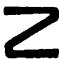
\includegraphics[keepaspectratio]{images/part001_f9c264f7.jpg}}

\begin{enumerate}
\def\labelenumi{(\arabic{enumi})}
\setcounter{enumi}{3}
\tightlist
\item
  例 (3) 表明 \(\mathbf{Z}\) -模 \(\mathbf{Q}\) 是平坦且忠实的模，但不是忠实平坦的。
\end{enumerate}

命题 2. 设 E 是忠实平坦右 A-模， \(u: \mathbf{N}' \to \mathbf{N}\) 是左 A-模同态。为使 \(u\) 是单射（相应地满射、双射），必须且只需 \(1_{\mathbf{E}} \otimes u: \mathbf{E} \otimes_{\mathbf{A}} \mathbf{N}' \to \mathbf{E} \otimes_{\mathbf{A}} \mathbf{N}\) 是如此。

这是命题 1 的判别准则 (a) 的直接推论。

命题 3. 设 \(0 \to E' \to E \to E'' \to 0\) 是右 A-模的正合列。假设 \(E'\) 与 \(E''\) 都平坦，且其中一个是忠实平坦的。则 \(E\) 是忠实平坦的。

我们已知 E 是平坦的（§2 第 5 目，命题 5）。我们验证 E 具有命题 1 的性质 (b)。设 N 是左 A-模。由于 E'' 平坦，有正合序列

\[
0 \rightarrow \mathrm{E} ^ {\prime} \otimes_ {\mathrm{A}} \mathrm{N} \rightarrow \mathrm{E} \otimes_ {\mathrm{A}} \mathrm{N} \rightarrow \mathrm{E} ^ {\prime \prime} \otimes_ {\mathrm{A}} \mathrm{N} \rightarrow 0
\]

（§2 第 5 目，命题 4）。若 \(\mathbf{E} \otimes_{\mathbf{A}} \mathbf{N} = 0\) ，则 \(\mathbf{E}' \otimes_{\mathbf{A}} \mathbf{N}\) 与 \(\mathbf{E}'' \otimes_{\mathbf{A}} \mathbf{N}\) 都为零；由于模 \(\mathbf{E}', \mathbf{E}''\) 之一是忠实平坦的，这蕴含 \(\mathbf{N} = 0\) 。

